\documentclass[11pt,catalan,a4paper,authoryear,twoside]{book} 
\usepackage[utf8]{inputenc}
\usepackage[T1]{fontenc}
\usepackage[catalan]{babel}
\selectlanguage{catalan}
%\usepackage[applemac]{inputenc}
\usepackage{graphicx}
\usepackage{amsfonts,amsmath,amsthm,amssymb}
\usepackage{multirow,url,dcolumn}
%\usepackage{pifont}
%\usepackage{psfrag}
%\usepackage{epsfig}
\usepackage{pstricks,pst-plot,pst-node} % core PSTricks packages (loaded first)
\usepackage{pst-text} 
%\usepackage{arrayjob,multido,ifthen}
%\usepackage{slashbox}
%\usepackage{moreverb}

%\usepackage{varioref}
%\DeclareGraphicsRule{.emf}{bmp}{}{}
%\DeclareGraphicsExtensions{.pdf,.png,.jpg}
% Schema for thesis format
% --------------------------------------------------------------
\usepackage[Glenn]{fncychap}
\ChNumVar{\fontsize{76}{80}\usefont{OT1}{pzc}{m}{n}\selectfont}
\ChTitleVar{\raggedleft\Large\sffamily\bfseries}

\usepackage[vcentering,dvips,papersize={170mm,240mm},
total={130mm,200mm},includehead,includefoot]{geometry}
\usepackage[cam,width=17truecm,height=21truecm,center]{crop}


% Enumeration of chapters, sections and table of contents
% --------------------------------------------------------------
\addtocounter{tocdepth}{1}
\newcommand{\clearemptydoublepage}{\newpage{\pagestyle{empty}\cleardoublepage}}

% Headers and page numbers
% --------------------------------------------------------------
\usepackage{fancyhdr} % To add headers
\pagestyle{fancy}
\fancyhead{}

\fancyhead[RO]{\slshape\small \nouppercase{\rightmark}}
\fancyhead[LE]{\slshape\small \nouppercase{\leftmark}}
%\fancyfoot[RE,LO]{\upshape\tiny PRHLT-DSIC-UPV} %% REVISAR %%
\fancyfoot[C]{\thepage}

\usepackage[below]{placeins}
\renewcommand{\textfraction}{0.0}
\renewcommand{\topfraction}{1.0}
\renewcommand{\bottomfraction}{1.0}
\renewcommand{\floatpagefraction}{1.0}
\usepackage{afterpage}
\usepackage{float}
\usepackage[bf]{caption}
\usepackage{subcaption}
%\renewcommand{\captionfont}{\linespread{0.95}\small}
\setcaptionmargin{1cm}
\setlength{\belowcaptionskip}{2mm}

%\usepackage[hang,raggedright,nooneline]{subfigure}
%\renewcommand{\subcapsize}{\linespread{.2}\scriptsize}
%\renewcommand{\subfigcapskip}{0mm}
%\renewcommand{\subfigbottomskip}{0mm}

%%%%%%%%%%%%%%%%%%%%%%%%%%%%%%%%%%%%%%%%%%%%%%%%%%%%%%%%%%%%%%%%%%


\usepackage{listings}

\usepackage{color}
\definecolor{gray}{rgb}{0.4,0.4,0.4}
\definecolor{darkblue}{rgb}{0.0,0.0,0.6}
\definecolor{cyan}{rgb}{0.0,0.6,0.6}

\lstset{
  basicstyle=\ttfamily,
  columns=fullflexible,
  showstringspaces=false,
  commentstyle=\color{gray}\upshape
}


% Chapter header format
% --------------------------------------------------------------
\makeatletter
\def\@makechapterhead#1{%
  \vspace*{30\p@}%
  {\parindent \z@ \raggedleft \reset@font
          \Large \scshape \@chapapp{} \thechapter
        \par\nobreak
        \interlinepenalty\@M
    \Huge \bfseries #1\par\nobreak
    %\vspace*{1\p@}%
    \hrulefill
    \par\nobreak
    \vskip 55\p@
  }}

\def\@makeschapterhead#1{%
  %\vspace*{10\p@}%
  {\parindent \z@ \raggedleft \reset@font
            \scshape \vphantom{\@chapapp{} \thechapter}
        \par\nobreak
        \interlinepenalty\@M
    \Huge \bfseries #1\par\nobreak
    %\vspace*{1\p@}%
    %\hrulefill
    \par\nobreak
    \vskip 40\p@
  }}
\makeatother

\graphicspath{{images/}}

\definecolor{DarkGreen}{cmyk}{.9,0,.9,.7}

\renewcommand{\vec}[1]{\ensuremath{\boldsymbol{#1}}}
\newcommand{\x}{\vec{x}}
\newcommand{\y}{\vec{y}}
\newcommand{\vu}{\vec{u}}
\newcommand{\vv}{\vec{v}}
\newcommand{\X}{X}
\newcommand{\Y}{Y}
\newcommand{\U}{U}
\newcommand{\V}{V}
\DeclareMathOperator*{\argmax}{argmax}
\DeclareMathOperator*{\argmin}{argmin}

%\renewcommand{\thefootnote}{\alph{footnote}} % To change footnote enumeration from number to letters

\newcommand{\marginnote}[2][0] {
 \marginpar{\vspace{#1}
             \begin{minipage}{20mm}
                \setlength{\baselineskip}{10pt}
                \flushleft
                \begin{scriptsize} {#2} \end{scriptsize}
             \end{minipage}}
}

\title{
  \begin{small}
    UNIVERSITAT POLITÈCNICA DE VALÈNCIA\\
  \vspace{0.25cm}
    ESCOLA TÈCNICA SUPERIOR D'ENGINYERIA INFORMÀTICA\\
  \vspace{0.25cm}
    DEPARTAMENT DE SISTEMES INFORMÀTICS I COMPUTACIÓ\\
  \end{small}
  \vspace{1cm}
  \begin{center}
    \mbox{
\includegraphics[width=6cm]{upv_val}}
  \end{center}
  \vspace{1cm}
  \begin{LARGE}
    % Title Page
    Quantificació de les millores en la segmentació del cos central del text manuscrit utilitzant aprenentatge supervisat
  \end{LARGE}
}
\author{
  \vspace{1cm}
  \small{Projecte Final de Carrera - Enginyeria Informàtica}\\
  Joan Puigcerver i Pérez\\
  \\
  Supervisat per:\\
  Dr. Moisés Pastor i Gadea
}

\begin{document}

\frontmatter

\maketitle
\clearemptydoublepage

\newpage\thispagestyle{empty}

\vspace*{2in}
\begin{flushright}
{\large {\it 
Als meus pares per mai haver-me dit ``prou''.\\
A la meva germana per suportar-me\\
fent-li la punyeta.\\
A Anna per alegrar-me els dies i\\
acompanyar-me arreu del món.\\ 
A Adrià i Fernando per tots els riures\\
durant aquests cinc anys.\\
I a Moisés per la seva confiança\\
i oportunitats que han resultat\\
en aquest treball i m'han obert portes\\
a llocs increïbles.}}
\end{flushright}

\clearemptydoublepage

\tableofcontents

\clearemptydoublepage

\mainmatter

% 1. Introducció
%   1.1. Motivació
%   1.2. Reconeixement de formes
%   1.2. Reconeixement de text manuscrit offline
% 2. Tècniques de la segmentació del cos central
%   2.1. Aproximació heurística
%   2.2. Aproximació Supervised Learning
% 3. Corpus
% 4. Experimentació
%   4.1. Preprocés
%   4.2. Model de llenguatge
%   4.3. Aïllament de la normalització de la grandària
%   4.4. Resum de resultats
% 4. Conclusions

\chapter{Introducció}
\label{cap:int}

\section{Motivació}
Des de fa unes poques dècades, els ordinadors permeten emmagatzemar una àmplia varietat d'informació de manera fiable i replicada per a que puga sobreviure al pas del temps, mantenir-la organitzada per a que siga fàcilment utilitzable i fer-la accessible arreu del món i quasi universalment. Però durant segles, l'única forma de transmetre el coneixement i emmagatzemar-lo de manera més o menys segura ha sigut mitjançant l'escriptura. Precisament el fet de mantenir el coneixement en llibres, manuscrits primer i impresos després, que permeten la seva preservació i més fàcil difusió, ha sigut una de les principals bases de tot el desenvolupament del coneixement humà, especialment científic i tecnològic, arreu del món i és el principal motor pel qual avui gaudim d'unes millors condicions de vida que les dels nostres avantpassats.\\

Malauradament, els llibres manuscrits i impresos no sempre han tingut èxit en la seva missió de preservar el coneixement. Sols cal recordar el desastrós incendi de l'antiga Biblioteca d'Alexandria que provocà que milers d'obres d'autors de l'antiguitat es perderen per sempre. Ajudar a la preservació de la informació continguda en els llibres manuscrits i ajudar també a la cerca del contingut en aquests, són dos dels motius que van fer nàixer el reconeixement de text manuscrit (HTR, de l'anglès \emph{Handwriting Text Recognition}) a principis del segle XX.\\

A pesar de tot el progrés aconseguit en els últims anys pel Reconeixement de Text Manuscrit, aquest té encara molts problemes per resoldre causats perquè gran part de la variabilitat que es troba en les imatges que s'utilitzen per reconèixer el text dels llibres no aporta cap informació rellevant per a la classificació dels símbols representats i dificulta el seu reconeixement. Per exemple, un mateix autor no escriu un mateix símbol sempre de la mateixa forma, ni de la mateixa grandària i ni tan sols amb la mateixa orientació; i l'objectiu és que tots aquests diferents traços siguen classificats de la mateixa manera. Per això, un dels components fonamentals de qualsevol sistema de reconeixement de l'escriptura és la normalització d'aquesta imatge, un procés que tracta de reduir aquesta variabilitat.\\

Aquest projecte compara i quantifica les diferències entre dues alternatives per solucionar un dels problemes que forma part d'aquest procés de normalització: la segmentació del del cos central del text manuscrit. El cos central d'una línia de text manuscrit és aquella porció de la línia on resideix el cos central de cadascun dels símbols que formen el text. Les dues alternatives estudiades per a aquesta segmentació del cos central estan basades en un enfocament heurístic del problema, on un algorisme amb unes regles pre-establertes determina quina és la regió del cos central, i una altra basada en tècniques d'aprenentatge supervisat, on un humà ha segmentat manualment el cos central d'un conjunt d'imatges de mostra i ha entrenat el sistema per a que intente segmentar de manera semblant les noves imatges. Els detalls es veuran en el capítol \ref{cap:seg}.


\section{Reconeixement de formes}
El reconeixement de formes (de l'anglès \emph{Pattern Recognition}) és una branca de l'aprenentatge automàtic que té com a objectiu fer que una màquina (un ordinador) tinga la capacitat de discernir entre diferents objectes del seu entorn. El sistema pot percebre el seu entorn a partir de diferents sensors com poden ser càmeres fotogràfiques o de vídeo, micròfons, sensors làser, de temperatura, etc. L'objectiu és, a partir de les senyals obtingudes per aquests sensors, descobrir i atorgar una significat als diferents objectes representats en les senyals (típicament, assignar-los a una categoria) \cite{DH73}.\\

Existeixen dos grans grups de problemes de reconeixement de formes. El primer, com s'havia dit, consisteix en assignar una categoria a algun objecte representat per una imatge. Per exemple, donada una imatge que conté una lletra, decidir quina lletra hi ha representada. És diu d'aquests problemes que tenen un aprenentatge supervisat perquè al sistema se l'entrena amb senyals d'entrada prèviament etiquetades, de manera que puga aprendre quines són les propietats en el senyal que determinen la seva categoria.\\

En el segon grup, no és disposa de les categories assignades al senyal durant l'etapa d'entrenament. L'objectiu d'aquest grup és descobrir propietats en el senyal d'entrada. Per exemple, assignar una categoria automàtica a cadascuna de les senyals d'entrada (\emph{clustering}) o trobar un model (típicament probabilístic) que permeta representar les dades d'entrenament. \\

Són moltes les aplicacions que poden ser interpretats com un problema de reconeixement de formes, és per això, i gràcies a l'avanç en la tecnologia informàtica, que l'interès en aquest camp a crescut notablement en les darreres dècades. Algunes de les aplicacions del reconeixement de formes són:
\begin{itemize}
\item Aplicacions sobre el llenguatge humà: Reconeixement automàtic de text, reconeixement automàtic de la parla, traducció automàtica, etc.
\item Aplicacions sobre imatges: Reconeixement facial, detecció i classificació d'objectes, etc.
\item Medicina: Detecció de tumors, classificació de cromosomes, etc.
\item Física: Detecció i classificació de cossos celestes, detecció de partícules subatòmiques, etc.
\end{itemize}

En el cas de l'aprenentatge supervisat, que és el més estès i el que s'utilitzarà en una de les tècniques descrites en aquest treball per a la segmentació del cos central (veure secció \ref{sec:seg_nn}), el procés de reconeixement es fa seguint el següent procediment (veure figura \ref{fig:rf}).

\begin{enumerate}
\item \textbf{Preprocessament}: Al senyal se li apliquen diferents transformacions que tenen com a objectiu eliminar la informació no rellevant per a la classificació.
\item \textbf{Extracció de característiques}: El resultat del preprocessament sol ser un senyal amb un alt nombre de dimensions i això dificulta l'estimació dels models per a la classificació. Per això, es tracta de reduir aquest nombre de dimensions extraient el que s'anomenen ``característiques'' del senyal (informació més rellevant per a representar-lo), que no són més que una representació del senyal en un espai menor de dimensions.
\item \textbf{Aprenentatge}: S'aprèn un model per a classificar la senyal amb la informació aportada per les característiques de la senyal d'entrada i el coneixement a priori sobre les dades i la tasca (categoria del senyal, probabilitats de les categories, etc). Aquesta fase sols és utilitzada durant l'aprenentatge del model.
\item \textbf{Classificació}: Una vegada l'aprenentatge està complet, s'utilitzen les característiques del senyal i el model obtingut en el pas anterior per a predir la categoria d'una nova observació del senyal.
\end{enumerate}

\begin{figure}
\centering
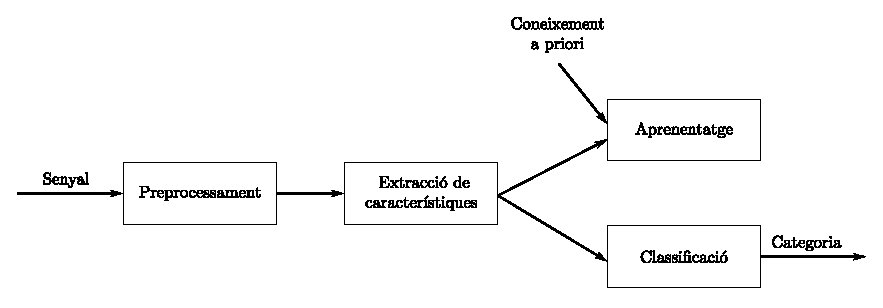
\includegraphics[width=\textwidth]{images/rf.eps}
\caption{Esquema d'un sistema de reconeixement de formes.}
\label{fig:rf}
\end{figure}

L'objectiu de l'aprenentatge supervisat pot interpretar-se com l'estimació d'una funció $g$ amb perfil $g : X \rightarrow C$, on $X$ és l'espai de característiques del senyal i $C$ el conjunt de categories; de manera que es minimitzen els errors de classificació per a un conjunt de dades d'entrenament $D = \{(x_1, c_1), (x_2, c_2), \ldots, (x_n, c_n)\}$ on $x_i$ és són les característiques obtingudes d'una mostra del senyal d'entrada i $c_i$ la seva categoria assignada. \\

La millor manera de construir aquesta funció és assignant la categoria $\hat{c}$ que maximitza la probabilitat de que les característiques del senyal observat representen aquesta categoria \cite{DH73}.
\begin{equation}\label{eq:bayes_classif}
g(x) = \argmax_{\forall c \in C} p(c|x) = \hat{c}
\end{equation}

L'equació \ref{eq:bayes_classif} pot escriure's de nou utilitzant el Teorema de Bayes segons l'equació \ref{eq:bayes_classif_v2} \cite{Bayes01011763}.

\begin{equation}\label{eq:bayes_classif_v2}
g(x) = \argmax_{\forall c \in C} \frac{p(c,x)}{p(x)} = \argmax_{\forall c \in C} \frac{p(x|c) p(c)}{p(x)} = \argmax_{\forall c \in C} p(x|c) p(c)
\end{equation}

Si es conegueren les distribucions exactes de $p(x|c)$ i $p(c)$, el problema de classificació quedaria resolt. Malauradament aquestes distribucions de probabilitat són desconegudes en les aplicacions reals i la major part del treball es concentra en trobar unes bones aproximacions d'aquestes a partir de les dades d'entrenament.

\section{Reconeixement de text manuscrit}
El reconeixement de text manuscrit (HTR, de l'anglès \emph{Handwriting Text Recognition}) començà a desenvolupar-se a principis del segle XX amb l'aparició de dispositius que permetien classificar dígits o caràcters manuscrits sobre sensors d'una determinada forma \cite{Goldberg1914}. A mitjans del segle XX aparegueren els primers dispositius que permetien introduir el resultat d'aquesta classificació en un ordinador \cite{10.1109/AFIPS.1957.60} i fins i tot sistemes que eren capaços de reconèixer paraules manuscrites aïllades \cite{Harmon1962}. Aquests primers dispositius estaven limitats per el desenvolupament tècnic d'aquell temps i solien necessitar-se dispositius especials sobre els que escriure el text. No era possible reconèixer el text d'un document manuscrit existent (com un llibre o un formulari). Fou més tard i gràcies a l'expansió de la informàtica quan els sistemes HTR començaren a adquirir la qualitat necessària per a aplicar-los en tasques de reconeixement real, com ara el reconeixement de dígits en xecs bancaris o el reconeixement de codis postals en el servei de correu.\\

Entre els sistemes HTR se'n diferencien dos tipus: el reconeixement \emph{online} i l'\emph{offline}. La diferència rau en el mètode en que el senyal d'entrada al sistema és adquirit. En els sistemes HTR \emph{online} el reconeixement es duu a terme en el mateix moment en el que s'escriu el text gràcies a l'ús de bolígrafs electrònics que capturen el moviment de la mà, la velocitat d'escriptura, la pressió sobre la superfície, etc. El reconeixement \emph{offline} es duu a terme una vegada el text ja ha sigut escrit sobre una superfície (típicament paper). Un escànner, càmera fotogràfica o de vídeo obté llavors una imatge de la superfície que conté el text a reconèixer i aquest és el senyal a utilitzar pel sistema de reconeixement. Degut a que en el reconeixement \emph{online} es disposa d'informació temporal que no està disponible en el reconeixement \emph{offline}, es considera que el primer és un problema més senzill de resoldre (aconseguir sistemes amb un menor error de reconeixement).\\

Una altra divisió en les tasques de reconeixement de text, és si aquest es troba segmentat o és continu. En el reconeixement de text segmentat, cadascun dels símbols a reconèixer es troba ben separat de la resta (figura \ref{fig:text_segmentat}). No ocorre el mateix en el reconeixement de text continu, on pot haver diferents símbols units per un mateix traç (figura \ref{fig:text_continu}). En el sistema d'escriptura occidental, el text continu és el més habitual en el text manuscrit. El cas continu es considera més difícil ja que la forma d'un símbol depèn fortament dels seus adjacents i l'unió de certs símbols pot ocasionar ambigüitat i requereix més context (per exemple, ``rn'' o ``m'', ``vv'' o ``w'', etc).\\

\begin{figure}
\centering
\begin{subfigure}[b]{0.4\textwidth}
\centering

\includegraphics[width=\textwidth]{images/reconeixement_segmentat.eps}
\caption{Text segmentat}\label{fig:text_segmentat}
\end{subfigure}
~
\begin{subfigure}[b]{0.4\textwidth}
\centering

\includegraphics[width=\textwidth]{images/reconeixement_continu.eps}
\caption{Text continu}\label{fig:text_continu}
\end{subfigure}
\caption{Dos exemples d'una paraula escrita amb text segmentat i continu.}
\end{figure}

Finalment, hi ha sistemes que estan restringits al reconeixement de paraules aïllades o de línies de text. El primer cas pot ser d'utilitat en aplicacions com el reconeixement d'adreces en cartes postals o el reconeixement de text en formularis, però resulta poc útil en el cas de voler reconèixer més d'una paraula (com les línies d'un llibre), ja que el context de cada paraula facilita el seu reconeixement i no aprofitar aquesta informació significa un major nombre d'errors.\\

Els principals problemes, per tant, als que s'enfronta un bon sistema de reconeixement del text manuscrit són:
\begin{itemize}
\item \textbf{Soroll en les imatges}: la imatge capturada pot contenir soroll que depèn de l'eina d'escriptura (un bolígraf o un llapis), la superfície (paper o cartró) o el tipus d'eina d'adquisició i la seva qualitat.
\item \textbf{Diferents estils d'escriptura}: el mateix símbol és escrit de moltes formes, no sols depenent de l'autor, sinó també depenent del seu estat d'ànim, rapidesa en l'escriptura, context en el que es situa el símbol, etc.
\end{itemize}

L'etapa de preprocessament que es descrivia abans intenta per una banda eliminar o reduir el soroll en les imatges, i per altra, reduir les diferències en els estils d'escriptura. La correcta segmentació del cos central del text és important per aplicar certes transformacions que tenen com a objectiu la reducció d'aquest segon problema.\\

Aquest projecte s'ha realitzat en un context de reconeixement de text manuscrit \emph{offline}, continu i de línies completes. No obstant això, els mètodes estudiats en aquest projecte per a la segmentació del cos central del text poden ser utilitzats igualment en un entorn de text segmentat i/o paraules aïllades.\\

Podem aplicar l'equació \ref{eq:bayes_classif} que s'havia presentat anteriorment per solucionar el problema del reconeixement de text \emph{offline}. Suposem que disposem d'una imatge $I$ que conté cert text, llavors l'objectiu és trobar la seqüència de símbols $\hat{s} = s_1, s_2, \ldots, s_N$ que maximitza la probabilitat de que aquests símbols siguen els representats en la imatge $I$.

\begin{equation}\label{eq:}
\hat{s} = \argmax_{s \in \Sigma^*} p(s|I)
\end{equation}

En el cas del reconeixement de text \emph{offline} i continu, típicament s'extreu una seqüència de vectors de característiques $\vec{x} = \vec{x}_1, \vec{x}_2, \ldots \vec{x}_T$ a partir de la imatge $I$. Aquests vectors s'extreuen a partir d'una finestra lliscant d'anàlisi que travessa tota la imatge. Per a cada posició on es fixa aquesta finestra, s'extreu un vector de característiques. La figura \ref{fig:finestra_lliscant} mostra aquesta finestra. Per tant, el reconeixement es reduiria a trobar la seqüència $\hat{s}$ que maximitza la probabilitat en  \ref{eq:bayes_classif}

\begin{equation}\label{eq:bayes_classif_vectors}
\hat{s} = \argmax_{s \in \Sigma^*} p(s|\vec{x}) = \argmax_{s \in \Sigma^*} p(\vec{x}|s) p(s) %= \argmax_{s \in \Sigma^*} p(\vec{x}_1, \vec{x}_2, \ldots \vec{x}_T | s) p(s)
\end{equation}

\begin{figure}
\centering

\includegraphics[width=\textwidth]{images/finestra_lliscant.eps}
\caption{Finestra lliscant d'anàlisi en una imatge}
\label{fig:finestra_lliscant}
\end{figure}

Habitualment, tant en entorns de reconeixement de text com de veu, la distribució a posteriori $p(\vec{x}|s)$ es modela utilitzant Models Ocults de Markov (HMM, de l'anglès \emph{Hidden Markov Models}) i Models de Mixtures Gaussianes (GMM, de l'anglès \emph{Gaussian Mixture Models}) \cite{huanghidden, jelinek1998statistical, ghahramani2001introduction} i $p(s)$ es modela utilitzant models de llenguatge de $n$-grames \cite{jelinek1998statistical,katz1987estimation,marti2001using}. Aquesta és l'aproximació que s'ha utilitzat en aquest projecte.
\clearemptydoublepage

\chapter{Tècniques de segmentació del cos central}
\label{cap:seg}
En aquest capítol s'introdueixen les dues tècniques per a la segmentació del cos central comparades en aquest projecte. La segmentació del cos central bàsicament tracta de trobar la frontera entre els ascendents, el cos central i els descendents en una imatge que conté text. Aquesta operació és de vital importància per a diferents tècniques del preprocessament, però sense dubte a la que més afecta és a la normalització del text, que al mateix temps, és una de les etapes del preprocessament que més efecte té sobre la qualitat del reconeixement. \\

Els ascendents i descendents són aquelles parts de la imatge on no resideix molta informació sobre el text representat, mentre que el cos central és aquella part on la major part de la informació resideix. Per exemple, pensem en el cas de les lletres ``o'', ``p'' i ``q''. El que diferència aquestes lletres, és bàsicament la línia vertical que es troba a l'esquerra del cercle, en el cas de la ``p'', i a la dreta, en el cas de la ``q''. Però la longitud d'aquesta línia vertical no aporta massa informació per a diferenciar entre aquestes 3 lletres. Sols és necessari saber si hi ha una línia vertical i on està situada aquesta. Si es traça una línia horitzontal per davall del cercle central de cadascuna de les lletres, aquella part de la imatge que resideix per baix, és el que s'anomenen \emph{descendents}. El mateix passa amb els símbols ``o'', ``b'' i ``d'', però ara la línia vertical es dirigeix cap amunt. En aquest cas, tot el que es troba per damunt del cercle central, serien els \emph{ascendents}. Finalment, en l'exemple anterior, anomenaríem \emph{cos central} al cercle que queda en el centre dels símbols. En la figura \ref{fig:ascendents_descendents_central} hi ha un exemple gràfic amb les zones diferenciades per a una paraula completa. \\

La línia que separa la zona d'ascendents del cos central s'anomena línia superior i la que separa el cos central dels descendents, inferior o línia base. \\

Una vegada s'ha segmentat el cos central de la imatge (s'han detectat les línies superiors i inferiors), el resultat es pot utilitzar per a normalitzar la grandària dels ascendents i descendents a una porció fixa del cos central, de manera que s'aconsegueix normalitzar l'altura de cadascun dels símbols representats a la imatge aconseguint que el cos central, on resideix la major part de la informació ocupe la major part de la imatge. Aquest procés de normalització és de vital importància per al reconeixement, ja que l'expressivitat dels models morfològics és limitada i resulta convenient que els vectors de característiques tinguen components el més significatives possibles. Per exemple, a la figura \ref{fig:finestra_lliscant} pot observar-se que gran part de la finestra lliscant, de la qual s'obtindrà el vector de característiques, està ocupada per blanc, que no aporta cap informació a l'hora de classificar el símbol.\\

\begin{figure}
\centering

\includegraphics[width=0.8\textwidth]{images/ascendents_descendents_central.eps}
\caption{Zones d'ascendents, cos central i descendents d'una paraula. Imatge cedida per \cite{Pastor07}}\label{fig:ascendents_descendents_central}
\end{figure}

\section{Aproximació heurística}
\label{sec:seg_heur}
L'algorisme que es descriu en aquesta secció per a detectar el cos central d'una imatge, fou presentat en \cite{Romero05} i \cite{Pastor07} i consisteix en les següents operacions.
\begin{enumerate}
\item La línia es segmenta en diferents parts que estan completament separades per espais blancs. Cadascuna d'aquestes parts serà normalitzada per separat. És important tenir en compte que l'objectiu no és fer un reconeixement del text de cadascuna d'aquestes parts, sinó segmentar el cos central del text de manera diferent en cadascuna d'aquestes per separat. La idea és que l'estil d'escriptura es conserva a cadascuna d'aquestes parts però pot variar d'una part a una altra.
\item Per a cada part del text, es detecten les línies base i superior de la imatge. Aquesta detecció es subdivideix en els següents passos:
\begin{enumerate}
\item Binarització de la imatge.
\item Suavitzat de la imatge original mitjançant l'algorisme Run-Length Smoothing Algorithm (RLSA).
\item Detecció de les vores superior i inferior de cada segment.
\item Càlcul de les rectes que millor s'ajusten a les fronteres superior i inferior, utilitzant la tècnica dels mínims quadrats.
\end{enumerate}
\end{enumerate}

La figura \ref{fig:pasos_segmentacio_heuristica} mostra tots els passos de la normalització heurística per a una imatge que conté una línia de text de mostra.\\

\begin{figure}
\centering
\begin{subfigure}[b]{0.8\textwidth}
\centering

\includegraphics[width=\textwidth]{images/pasos_segmentacio_heuristica_original.eps}
\caption{Imatge original.}\label{fig:pasos_segmentacio_heuristica_original}
\end{subfigure} \\
\begin{subfigure}[b]{0.8\textwidth}
\centering
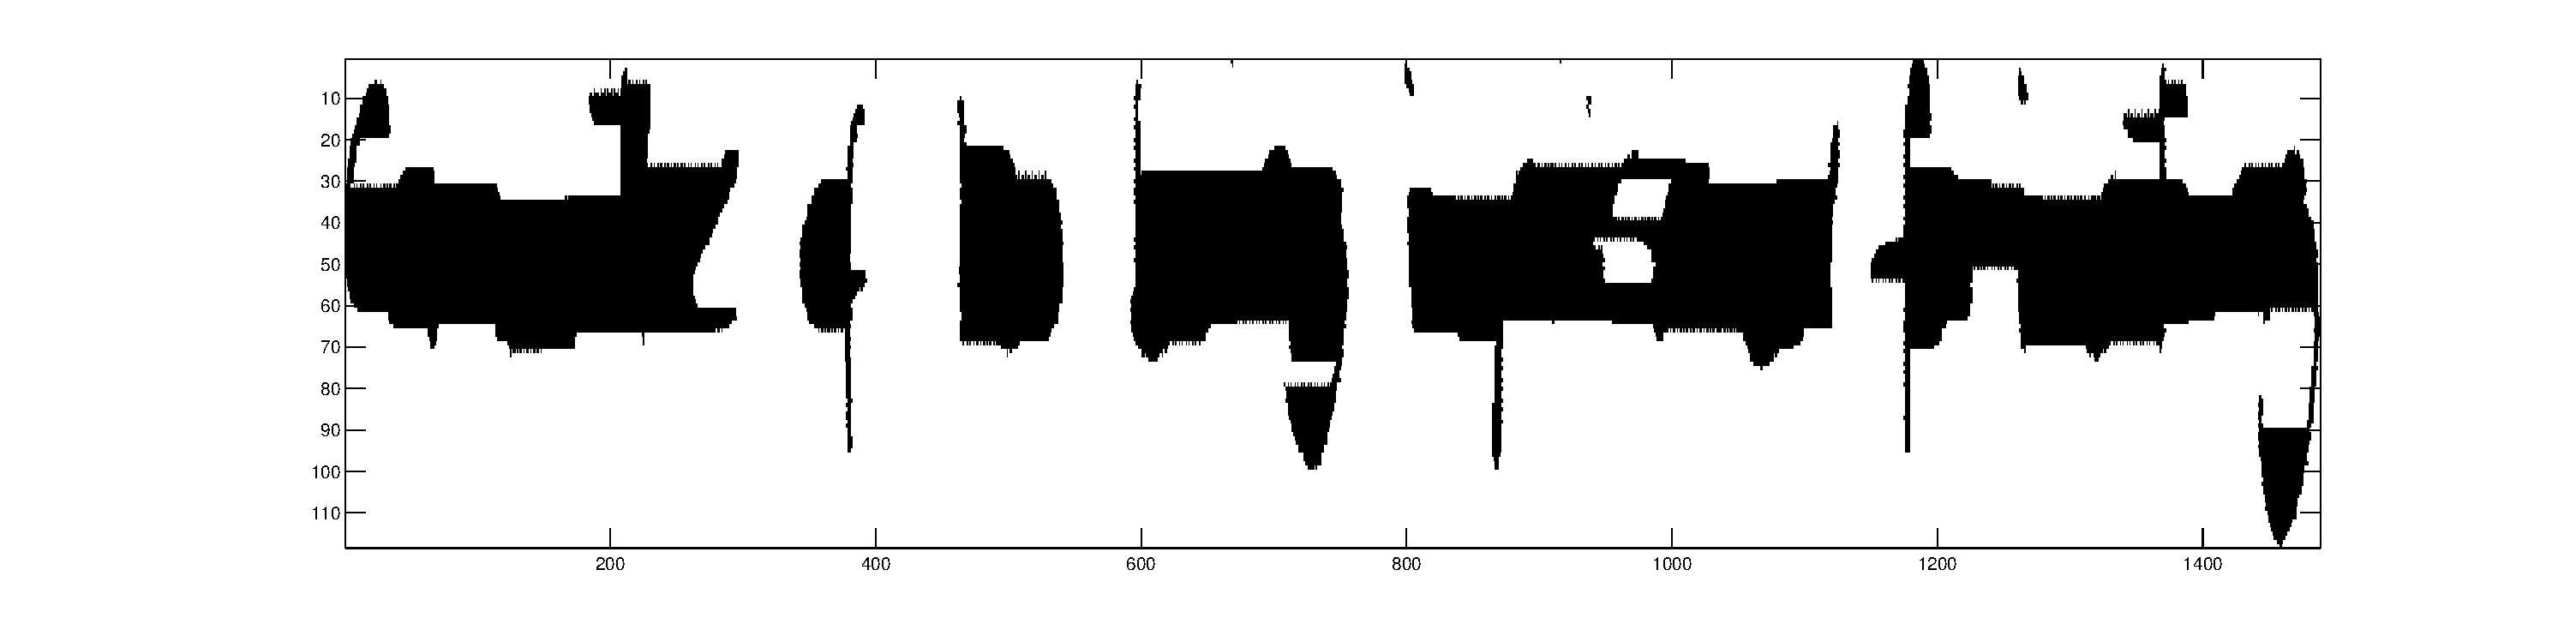
\includegraphics[width=\textwidth]{images/pasos_segmentacio_heuristica_rlsa.eps}
\caption{Resultat de l'algorisme RLSA.}\label{fig:pasos_segmentacio_heuristica_rlsa}
\end{subfigure}\\
\begin{subfigure}[b]{0.8\textwidth}
\centering

\includegraphics[width=\textwidth]{images/pasos_segmentacio_heuristica_vora_superior.eps}
\caption{Resultat de la detecció de la vora superior.}\label{fig:pasos_segmentacio_heuristica_sup}
\end{subfigure}\\
\begin{subfigure}[b]{0.8\textwidth}
\centering

\includegraphics[width=\textwidth]{images/pasos_segmentacio_heuristica_vora_inferior.eps}
\caption{Resultat de la detecció de la vora inferior.}\label{fig:pasos_segmentacio_heuristica_inf}
\end{subfigure}\\
\begin{subfigure}[b]{0.8\textwidth}
\centering
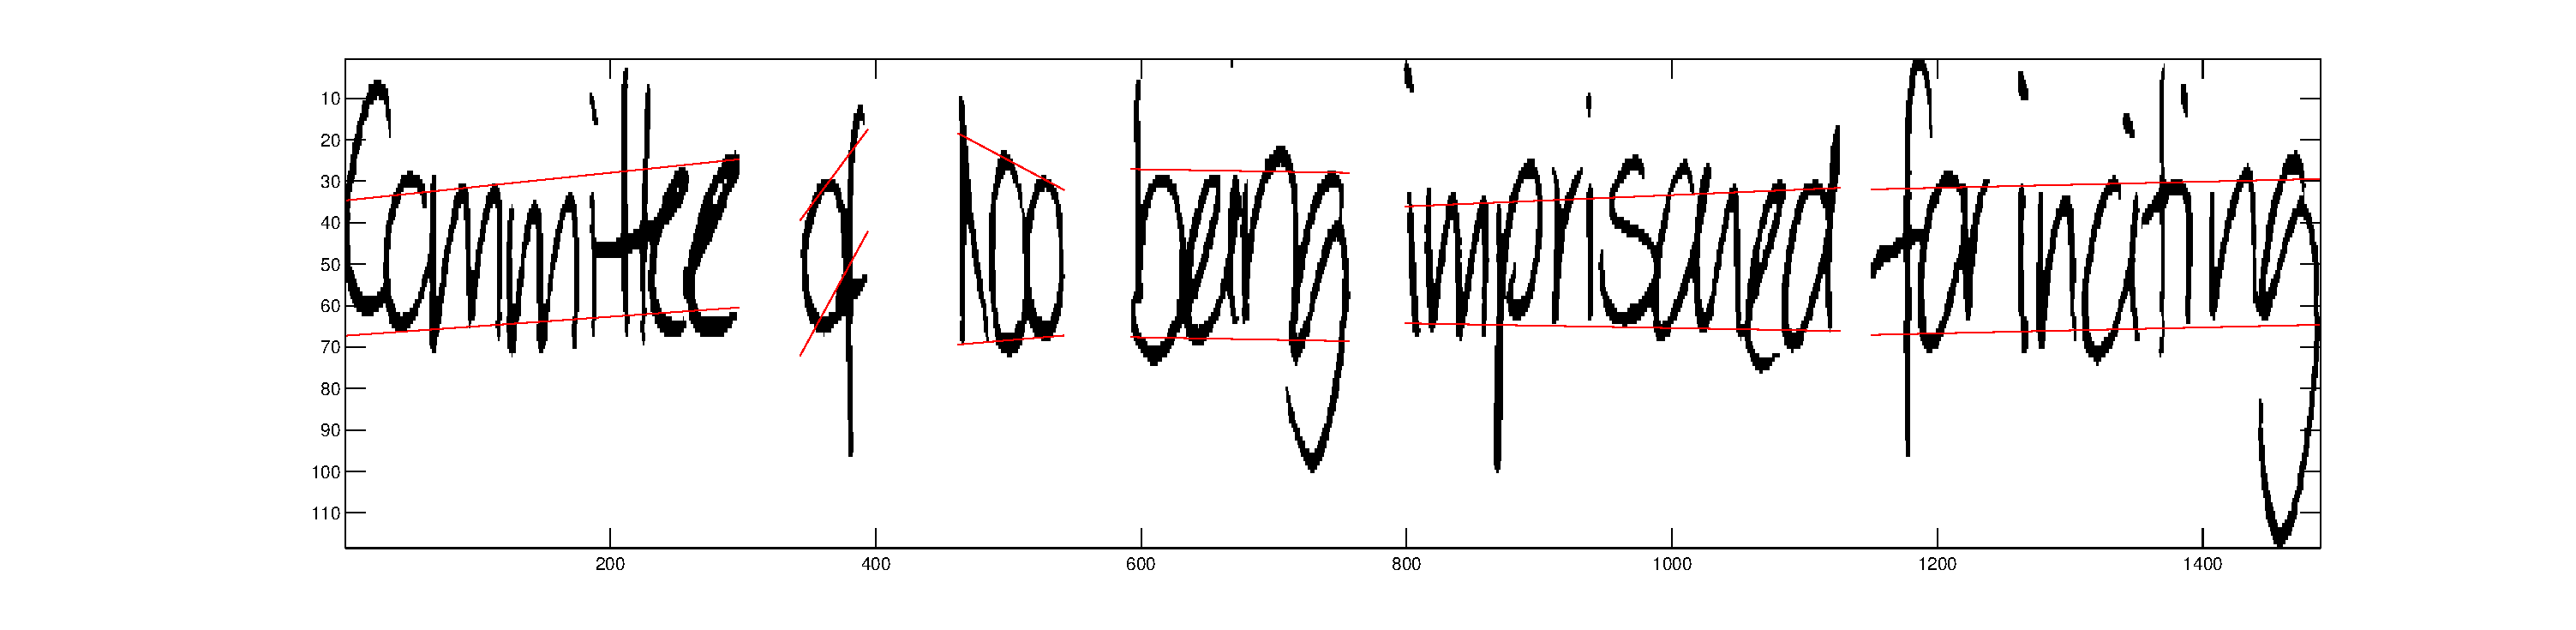
\includegraphics[width=\textwidth]{images/pasos_segmentacio_heuristica_final.eps}
\caption{Resultat final de la segmentació.}\label{fig:pasos_segmentacio_heuristica_final}
\end{subfigure}\\
\caption{Resultat de cada pas de la segmentació del cos central utilitzant l'algorisme heurístic.}\label{fig:pasos_segmentacio_heuristica}
\end{figure}

Aquesta aproximació assumeix que les línies inferiors i superiors poden ser aproximades a una recta amb molt poc d'error. Aquesta assumpció pot no complir-se en la realitat i per tant, pot obtenir una mala aproximació a les línies inferiors i superiors. Un altre inconvenient d'aquest mètode és el llindar que s'utilitza per a fer l'esborronat en l'algorisme RLSA. En aquest algorisme s'uneixen dos píxels negres en una mateixa fila sempre que la separació siga menor que un cert llindar. Aquest llindar pot fer-se fixe o relatiu a la imatge. Siga com siga, si no s'ajusta bé aquest llindar pot ocasionar problemes com els de la figura \ref{fig:pasos_mala_segmentacio}, que alhora fan malbé les diferents etapes del preprocessament que depenen de la segmentació del cos central, com per exemple la normalització de la grandària.

\begin{figure}
\centering
\begin{subfigure}[b]{0.25\textwidth}
\centering

\includegraphics[width=\textwidth]{images/do.eps}
\caption{}\label{fig:pasos_mala_seg_original}
\end{subfigure}
~
\begin{subfigure}[b]{0.25\textwidth}
\centering
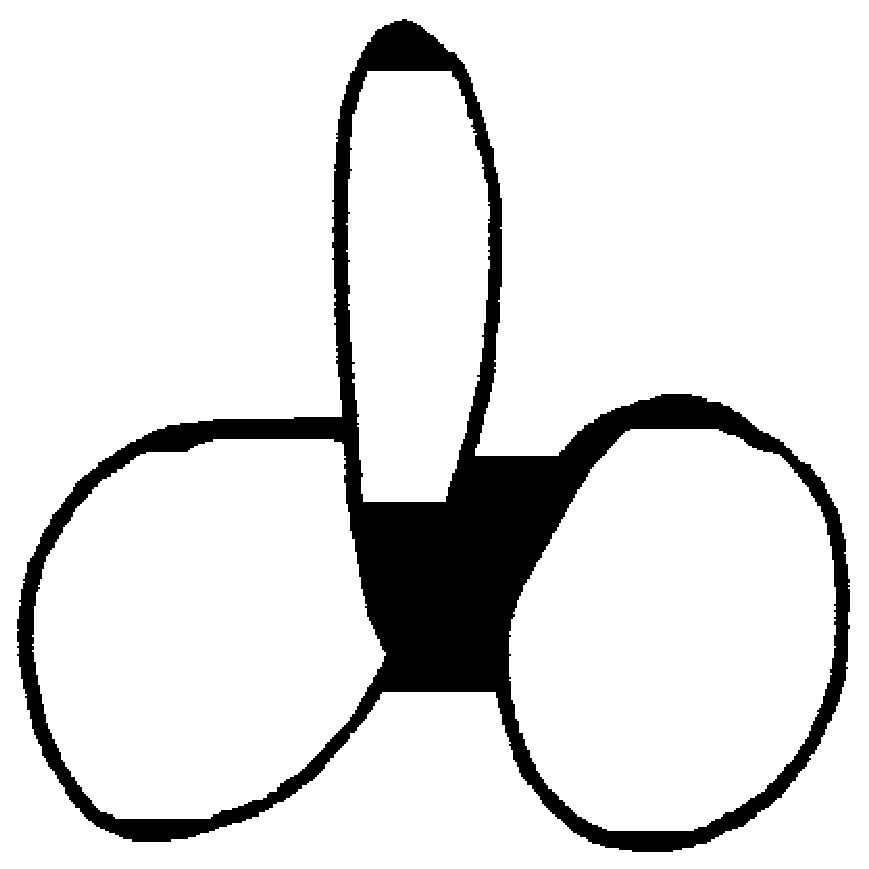
\includegraphics[width=\textwidth]{images/do_RLSA.eps}
\caption{}\label{fig:pasos_mala_seg_rlsa}
\end{subfigure}
~
\begin{subfigure}[b]{0.25\textwidth}
\centering

\includegraphics[width=\textwidth]{images/do_upcont.eps}
\caption{}\label{fig:pasos_mala_seg_sup}
\end{subfigure}\\
\begin{subfigure}[b]{0.25\textwidth}
\centering

\includegraphics[width=\textwidth]{images/do_lowcont.eps}
\caption{}\label{fig:pasos_mala_seg_inf}
\end{subfigure}
~
\begin{subfigure}[b]{0.25\textwidth}
\centering
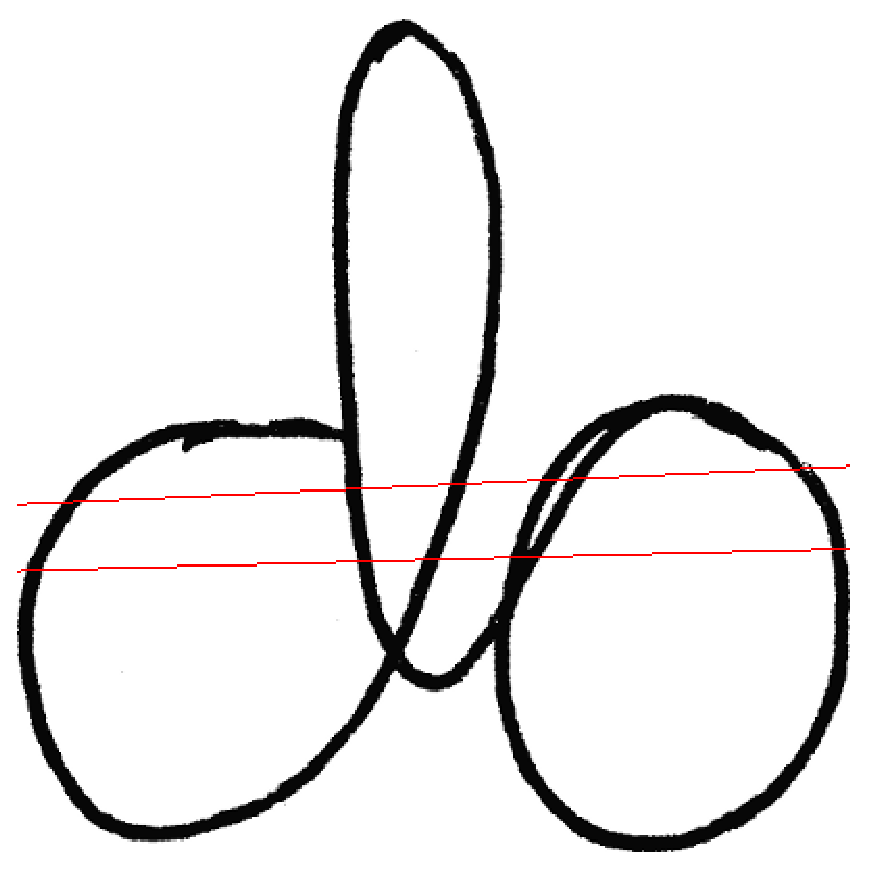
\includegraphics[width=\textwidth]{images/do_result.eps}
\caption{}\label{fig:pasos_mala_seg_lines}
\end{subfigure}
\\
\begin{subfigure}[b]{0.7\textwidth}
\centering
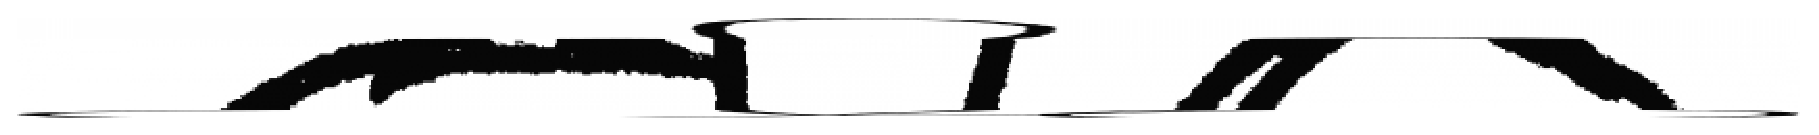
\includegraphics[width=\textwidth]{images/do_norm.eps}
\caption{}\label{fig:pasos_mala_seg_norm}
\end{subfigure}
\caption{Exemple d'una segmentació dolenta i els seus efectes. La figura \ref{fig:pasos_mala_seg_original} mostra la imatge original, la figura \ref{fig:pasos_mala_seg_rlsa} el resultat de l'algorisme RLSA, les figures \ref{fig:pasos_mala_seg_inf} i \ref{fig:pasos_mala_seg_sup} les vores inferior i superior detectades, la \ref{fig:pasos_mala_seg_lines} mostra les línies obtingudes a partir de les vores i finalment la figura \ref{fig:pasos_mala_seg_norm} el resultat de la normalització.}\label{fig:pasos_mala_segmentacio}
\end{figure}

\section{Aproximació utilitzant aprenentatge supervisat}
\label{sec:seg_nn}
Aquesta aproximació a la segmentació del cos central del text que fa ús d'aprenentatge supervisat fou presentada en \cite{DBLP:conf/pris/Gorbe-MoyaEZB08} i fa ús d'una xarxa neuronal multicapa per a classificar certs punts de la imatge en cinc classes: ascendent, línia superior, línia inferior, descendent i altres.\\

Per tal d'utilitzar aquesta tècnica s'han d'extreure un conjunt de punts extrems locals a partir del contorn de la imatge. Aquests punts s'obtenen de la següent manera.
\begin{enumerate}
\item Per a cada columna de la imatge, es busquen els punts de la frontera entre un píxel de fons (típicament blancs) i un píxel d'un símbol (típicament negres). D'aquesta manera s'obté el contorn de la imatge.
\item Es desplaça una finestra d'anàlisi sobre el contorn de la imatge i es seleccionen els píxels del contorn màxims i mínims locals. Un punt màxim és aquell en el qual la resta de píxels del contorn veïns es situen per davall. Un mínim, en el que es situen per sobre.
\end{enumerate}

Una vegada s'han obtingut els extrems locals, es situa una finestra de $W_w \times H_w$ píxels centrada en cada punt. A aquesta finestra se li aplica una distorsió d'ull de peix, de manera que els punts a prop del lloc d'interés queden ressaltats sobre aquells més llunyans i finalment es redueix a una grandària de $W_f \times H_f$ píxels. Aquesta serà l'entrada a la xarxa neuronal.\\

Per a entrenar la xarxa neuronal, s'utilitzen imatges amb els seus extrems locals classificats manualment, de manera que la xarxa neuronal aprèn a classificar un extrem local en una de les cinc classes mencionades anteriorment. Alternativament, per a facilitar l'entrenament del sistema, un humà pot corregir els punts classificats automàticament per un altre sistema més rudimentari per a la detecció de les línies de referència \cite{DBLP:conf/pris/Gorbe-MoyaEZB08}. Els detalls sobre l'entrenament de xarxes neuronals poden consultar-se en diverses fonts sobre aprenentatge automàtic \cite{DH73,bishop2006pattern,murphy2012machine}.\\

Per a segmentar el cos central d'una imatge de \emph{test}, es classifiquen tots els punts utilitzant la xarxa neuronal entrenada anteriorment. Com que la classificació feta per la xarxa neuronal pot ser sorollosa i pot classificar com a punts de les línies de referència píxels que en realitat no ho són, s'aplica un filtre a l'eixida de la xarxa neuronal de manera que tots els punts que són classificats com a ``ascendents'', ``descendents'', ``línia superior'' o ``línia base'' i no superen un cert llindar en la probabilitat emesa per la xarxa neuronal, són finalment classificats com a ``altres''. Llavors tots els punts pertanyents a una mateixa classe són utilitzats per a construir una polilínia per a cadascuna de les quatre línies de referència (els píxels classificats com ``altres'' no s'utilitzen).\\

La figura \ref{fig:comp_seg_mlp_result} mostra el resultat d'aplicar l'anterior algorisme a una imatge que conté text manuscrit. Els punts marcats són els extrems locals classificats, les línies delimiten les zones d'ascendents i descendents.\\

% COMPARACIÓ VISUAL ENTRE LES DUES TÈCNIQUES
\begin{figure}
\centering
\begin{subfigure}[b]{0.9\textwidth}
\centering

\includegraphics[width=\textwidth]{images/comp_seg_original.eps}
\caption{}\label{fig:comp_seg_original}
\end{subfigure}\\
% Resultat de la segmentació segons cada tècnica.
\begin{subfigure}[b]{0.9\textwidth}
\centering

\includegraphics[width=\textwidth]{images/comp_seg_heur_result.eps}
\caption{}\label{fig:comp_seg_heur_result}
\end{subfigure}\\
\begin{subfigure}[b]{0.9\textwidth}
\centering

\includegraphics[width=\textwidth]{images/comp_seg_mlp_result.eps}
\caption{}\label{fig:comp_seg_mlp_result}
\end{subfigure}\\
% Resultat de la normalització segons cada tècnica.
\begin{subfigure}[b]{0.9\textwidth}
\centering

\includegraphics[width=\textwidth]{images/comp_seg_heur_norm.eps}
\caption{}\label{fig:comp_seg_heur_norm}
\end{subfigure}\\
\begin{subfigure}[b]{0.9\textwidth}
\centering

\includegraphics[width=\textwidth]{images/comp_seg_mlp_norm.eps}
\caption{}\label{fig:comp_seg_mlp_norm}
\end{subfigure}
\caption{Imatge original (\ref{fig:comp_seg_original}), segmentació del cos central segons l'aproximació heurística i basada en aprenentatge supervisat (\ref{fig:comp_seg_heur_result}, \ref{fig:comp_seg_mlp_result}) i resultat de la normalització segons cada aproximació (\ref{fig:comp_seg_heur_norm}, \ref{fig:comp_seg_mlp_norm}). Figures \ref{fig:comp_seg_original}, \ref{fig:comp_seg_mlp_result} i \ref{fig:comp_seg_mlp_norm} cedides per \cite{DBLP:conf/pris/Gorbe-MoyaEZB08}.}\label{fig:comp_seg}
\end{figure}

Les figures \ref{fig:comp_seg_heur_result} i \ref{fig:comp_seg_mlp_result} mostren les diferències en les assumpcions que fan cadascun dels dos mètodes explicats. La major informació que aporta la detecció de les línies de referència utilitzant el mètode supervisat pot oferir clarament una millora significativa a l'hora d'aplicar el procés de normalització a la imatge. En els següents capítols s'explicarà com s'han quantificat aquestes diferències per demostrar que, efectivament, l'ús del mètode supervisat millora considerablement el reconeixement de text manuscrit.
\clearemptydoublepage

\chapter{Corpus}
\label{cap:corpus}
En aquest capítol es detallen les dades utilitzades per a realitzar els experiments que quantifiquen les diferències entre els dos mètodes descrits en el capítol \ref{cap:seg}.

\section{IAMDB}\label{sec:corpus_iamdb}
El corpus IAMDB\footnote{\url{http://www.iam.unibe.ch/fki/databases/iam-handwriting-database}} fou recopilat pel grup d'investigació \emph{Computer Vision and Artificial Intelligence} (FKI) dins del \emph{Institute of Computer Science an Applied Mathematics} (IAM), a l'Universitat de Berna. El corpus és d'accés gratuit per a propòsits de recerca i és un dels més utilitzats per al reconeixement de text manuscrit. La primera versió es presentà en la ICDAR (International Conference of Document Analysis and Recognition) el 1999 \cite{MB99}. El corpus és una transcripció manual del corpus Lancaster-Oslo-Bergen (LOB), descrit en la secció \ref{sec:corpus_lob}. Diferents paràgrafs del LOB es repartiren a un grup de persones que reescriviren el text manualment sense cap tipus de restricció en quant al tipus, estil o eina d'escriptura. En 2002, el text fou segmentat per línies i per paraules aïllades \cite{ZB02} i presentada l'última versió en la revista IJDAR \cite{MB02}. Els experiments realitzats en aquest treball utilitzaren la versió del corpus segmentada per línies.\\

La taula \ref{tab:iamdb_original} conté les estadístiques de la versió de 2002 del corpus IAMDB, que ha sigut utilitzada. El corpus original compta amb dos conjunts de validació. Per a aquest projecte, a l'igual que han fet altres autors \cite{bertolami2008ensemble, graves2009novel, espana2011improving}, s'ha utilitzat part del primer conjunt de validació per a ampliar els conjunts de test i el segon de validació, de manera que la distribució final utilitzada per a l'entrenament, validació i test dels sistemes ha sigut l'ex\-pre\-sa\-da en la taula \ref{tab:iamdb_used}. Aquests conjunts són totalment disjunts i on cada escriptor ha participat únicament en un dels conjunts. El corpus IAMDB fou utilitzat per a entrenar els models morfològics del reconeixedor de text.\\

\begin{table}
\centering
\begin{tabular}{|c|c|c|}
\hline
Conjunt & Línies & Escriptors \\
\hline
Train & 6161 & 283 \\
Validation 1 & 900 & 46 \\
Validation 2	 & 940 & 43 \\
Test & 1861 & 128\\
\hline
Total & 9862 & 500\\
\hline
\end{tabular}
\caption{Estadístiques del corpus IAMDB original.}\label{tab:iamdb_original}
\end{table}

\begin{table}
\centering
\begin{tabular}{|c|c|c|}
\hline
Conjunt & Línies & Escriptors \\
\hline
Train & 6161 & 283 \\
Validation & 920 & 56 \\
Test & 2781 & 161\\
\hline
Total & 9862 & 500\\
\hline
\end{tabular}
\caption{Estadístiques de la partició feta a partir del corpus IAMDB original.}\label{tab:iamdb_used}
\end{table}

La figura \ref{fig:iamdb_examples} conté algunes de les imatges que formen part de la versió corpus IAMDB utilitzada.
\begin{figure}
\centering
\begin{subfigure}[b]{0.9\textwidth}
\centering

\includegraphics[width=\textwidth]{images/iamdb_a01-000u-06.eps}
\end{subfigure}\\
\begin{subfigure}[b]{0.9\textwidth}
\centering

\includegraphics[width=\textwidth]{images/iamdb_c01-066-00.eps}
\end{subfigure}\\
\begin{subfigure}[b]{0.9\textwidth}
\centering

\includegraphics[width=\textwidth]{images/iamdb_p06-248-00.eps}
\end{subfigure}\\
\caption{Exemples de línies de text extretes del corpus IAMDB.}\label{fig:iamdb_examples}
\end{figure}

% ======================================================================
% CORPUS BROWN
\section{Brown}\label{sec:corpus_brown}
El Corpus Estàndard d'Anglès Americà del Present, o simplement corpus Brown, va ser presentat originalment el 1961\cite{francis1979brown} per la Universitat de Brown i conté 500 textos d'aproximadament 2000 paraules cadascun, escrites en anglès americà actual i un total de 1.014.312 paraules entre tots els textos. El corpus conté informació sobre les categories de cada paraula en els textos, però aquesta informació no fou utilitzada per al desenvolupament d'aquest projecte. La taula \ref{tab:corpus_lm} conté un resum dels textos continguts en el corpus Brown. Aquest corpus fou utilitzat per a construir el model del llenguatge utilitzat en els experiments.

% ======================================================================
% CORPUS LOB
\section{Lancaster-Oslo-Bergen}\label{sec:corpus_lob}
El corpus Lancaster-Oslo-Bergen (LOB) fou recopilat i presentat el 1986\cite{johansson1986tagged} per investigadors de la Universitat de Lancaster, la Universitat d'Oslo i el \emph{Norwegian Computing Centre for the Humanities}, en Bergen. El corpus fou recopilat com una alternativa en anglès britànic al corpus de la Universitat de Brown, descrit en la secció \ref{sec:corpus_brown}, que fou desenvolupat a partir de textos en anglès americà. El LOB conté 500 textos d'unes 2000 paraules aproximadament i aproximadament un milió de paraules en tot el corpus. Cada paraula del corpus fou anotada posteriorment en categories, encara que aquesta informació no ha sigut utilitzada per al desenvolupament del projecte. La taula \ref{tab:corpus_lm} conté un resum dels textos continguts en el corpus LOB. Part d'aquest corpus fou utilitzat per a construir el model del llenguatge dels experiments. S'exclogueren aquells texts que s'havien utilitzat per transcriure les línies de text de \emph{test} del corpus IAMDB.

% ======================================================================
% CORPUS WELLINGTON
\section{Wellington}\label{sec:corpus_wellington}
El corpus Wellington d'Anglès escrit de Nova Zelanda, o corpus Wellington, fou presentat el 1993\cite{bauer1993manual} per la Universitat Victoria de Wellington, a Nova Zelanda, i fou desenvolupat a partir de textos escrits en l'anglès utilitzat a Nova Zelanda. El corpus es desenvolupà per a fer-lo comparable als corpus de LOB i Brown descrits anteriorment (seccions \ref{sec:corpus_brown} i \ref{sec:corpus_lob}). Conté també 500 textos de diferents categories, d'unes 2000 paraules cada text i al voltant d'un milió de paraules en tot el corpus. La taula \ref{tab:corpus_lm} conté un resum dels tres corpus utilitzats. Aquest corpus fou utilitzat per a construir el model del llenguatge utilitzat en els experiments.

\begin{table}
\centering
\begin{tabular}{|c|l|c|c|c|}
\hline
Categoria & Descripció & Brown & LOB & Wgton\\
\hline
A & Premsa: reportatges & 44 & 44 & 44\\
B & Premsa: editorial & 27 & 27 & 27\\
C & Premsa: ressenyes & 17 & 17 & 17\\
D & Religió & 17 & 17 & 17\\
E & Habilitats, oficis i aficions & 36 & 38 & 38\\
F & Tradició popular & 48 & 44 & 44\\
G & Belles lletres, biografia, assajos & 75 & 77 & 77\\
H & Miscel·lània & 30 & 30 & 30\\
J & Escrits científics & 80 & 80 & 80\\
K & Ficció general & 29 & 29 & 29\\
L & Ficció de misteri i policiaca & 24 & 24 & 24\\
M & Ciència Ficció & 6 & 6 & 6\\
N & Ficció d'aventures i de l'oest & 29 & 29 & 29\\
P & Històries d'amor i romàntiques & 29 & 29 & 29\\
R & Humor & 9 & 9 & 9\\
\hline
Total & & 500 & 500 & 500\\
\hline
\end{tabular}
\caption{Resum dels textos continguts en els corpus Brown, LOB i Wellington.}\label{tab:corpus_lm}
\end{table}
\clearemptydoublepage

\chapter{Experimentació} 
\label{cap:exp}
La principal tasca d'aquest projecte fou la de dissenyar els experiments de manera que els resultats foren el més possiblement comparables, de manera que l'única diferència que hi hagués entre el reconeixement emprant els dos mètodes fou la de la segmentació del cos central del text en les imatges. D'aquesta manera es pot conèixer exactament quines són les diferències quantitatives entre els dos mètodes, calculant la diferència en l'error de reconeixement obtingut a l'emprar les dues alternatives.\\

A banda de la publicació original on s'explicava l'aproximació que utilitza aprenentatge supervisat per a la segmentació del text \cite{DBLP:conf/pris/Gorbe-MoyaEZB08}, els mateixos autors publicaren en la revista \emph{IEEE Transactions on Pattern Analysis and Machine Intelligence} (PAMI), el 2011, una comparativa entre dos estratègies per a la modelització dels models morfològics. Una basada únicament en HMM i l'altra un híbrid entre HMM i ANN \cite{espana2011improving}. L'interessant d'aquesta publicació per a l'objectiu d'aquest projecte és que utilitzava la segmentació del cos central supervisada (secció \ref{sec:seg_nn}) en ambdós casos i donava més detalls sobre l'entrenament complet del reconeixedor (model de llenguatge, models morfològics, etc) que no pas l'article original on s'explica la segmentació del cos central utilitzant aprenentatge supervisat.\\

El disseny dels experiments ací descrits busca reproduir els resultats publicats en \cite{espana2011improving} del reconeixedor basat únicament en HMM utilitzant la segmentació del cos supervisada i comparar-los en un altre reconeixedor basat també en HMM i utilitzant la mateixa segmentació.

\section{Preprocessament de les imatges}
En els dos reconeixedors entrenats, s'aplicà el següent procés de preprocessament a les línies de text d'IAMDB.
\begin{enumerate}
\item Neteja de la imatge. L'objectiu d'aquesta etapa és la de netejar el soroll en les imatges utilitzades. La tècnica utilitzada fou la descrita en FALTA CITA.%\ref{}.
\item Correcció \emph{slant}. L'objectiu d'aquesta etapa és la de corregir l'angle 
\item Correcció \emph{slope}
\item Segmentació del cos central. Única part del preprocessament que canviava respecte als dos reconeixedors entrenats. En un s'utilitza la tècnica descrita en la secció \ref{sec:seg_heur} i en el segon la descrita en la secció \ref{sec:seg_nn}.
\item Normalització de l'altura d'ascendents i descendents
\item Extracció de característiques
\end{enumerate}

\section{Model del llenguatge}

\section{Model morfològic}

\begin{table}
\centering
\begin{tabular}{cc|c|c|c|}
\cline{3-5}
& & \multicolumn{3}{c|}{Components de la mixtura} \\
\cline{3-5}
& & 16 & 32 & 64 \\ 
\cline{1-5}
\multicolumn{1}{|c|}{\multirow{3}{*}{Nombre mitjà d'estats}} & 7 &  54.91 & 46.75 & 42.84 \\
\cline{2-5}
\multicolumn{1}{|c|}{} & 8 &  54.24 & 46.08 & \textbf{42.21} \\
\cline{2-5}
\multicolumn{1}{|c|}{} & 9 &  54.41 & 47.73 & 44.53 \\
\cline{1-5}
\end{tabular}
\caption{WER en el conjunt de validació utilitzant diferents paràmetres per a l'estimació dels HMM utilitzant la segmentació heurística.}\label{table:estimacio_parametres_HMM}
\end{table} 

\section{Postprocessament al reconeixement}
\clearemptydoublepage

\chapter{Conclusions}
\label{cap:con}

La taula \ref{tab:summary} situa els resultats obtinguts en aquest treball en comparació amb resultats obtinguts prèviament en la mateixa tasca de reconeixement.\\

\begin{table}
\begin{center}
\begin{tabular}{|l|c|c|}
\hline
& Validació & Test \\\hline\hline
Bertolami et al. \cite{bertolami2008hidden} & \textbf{30.98} & \textbf{35.52} \\\hline
España Boquera et al. \cite{espana2011improving} & 32.80 & 38.80  \\\hline
Seg. Supervisada & 32.99 & 40.08 \\\hline
Seg. Heurística & 38.74 & 45.54 \\\hline
\end{tabular}
\caption{Comparació del WER de les alternatives estudiades amb altres publicacions.}\label{tab:summary}
\end{center}
\end{table}

En aquesta taula s'observa que els resultats obtinguts a partir del sistema que empra una segmentació del cos central basada en aprenentatge supervisat no correspon als resultats obtinguts en la publicació. Això és degut a que, a pesar d'intentar replicar els experiments amb el major detall possible i comptar amb la col·laboració dels autors de l'article, hi ha nombrosos detalls sobre l'experimentació publicada que eren desconeguts i/o no van poder ser replicats. D'ací aquesta petita diferència en les mesures obtingudes.\\

Més important encara, s'observa que l'utilització d'una segmentació del cos central del text manuscrit utilitzant aprenentatge supervisat redueix un $11.99\%$ el WER respecte a l'alternativa tradicional basada en un enfocament heurístic, en la tasca de reconeixement del corpus IAMDB, un important corpus utilitzat a l'hora de mesurar els errors en les transcripcions dels sistemes de reconeixement automàtic de text manuscrit.\\

Queda per tant comprovada la hipòtesi que es presentava al descriure les diferències entre els dos enfocaments per a la segmentació del cos central del text manuscrit: l'ús d'una tècnica basada en aprenentatge supervisat millora significativament la segmentació heurística. Aquesta millora a sigut quantificada satisfactoriament a pesar de les dificultats a l'hora de reproduir els detalls de les experimentacions publicades amb anterioritat i sols queda per tant fer front a la qüestió de si aquesta millora compensa el cost econòmic i temporal d'utilitzar aquesta tècnica basada en aprenentatge supervisat per a sistemes reals.
\clearemptydoublepage

\bibliographystyle{alpha}
\bibliography{memoria}

\listoffigures
\listoftables

\end{document}

